\chapter{Phonon Anomalies in LSCO+O}

\section{Origin of the phonon anomaly}
Phonon anomalies in materials can, in general, happen for a number of reasons. The Cu-O bond-stretching phonon anomaly in LSCO does not seem to be caused by any of the conventional phenomena, and a relationship to novel charge modes has been proposed. One such charge mode is fluctuations of stripe order. The appeal of this interpretation is the near impossibility of measuring dynamic charge stripes directly. The phonon anomaly could thus provide an indirect way of investigating the elusive properties of dynamic charge stripes. Given the hypothesis that the phonon anomaly and dynamic charge stripes are related, what are then the possible mechanisms of the coupling? A couple of scenarios are given in Figure \ref{fig:anomaly_2d} and \ref{fig:anomaly_1d}.

The charge oscilation was introduced by \citeauthor{Kaneshita2002}\cite{Kaneshita2002} in a theoretical study of stripes coupling to the phonon. The Kohn anomaly picture was introduced in context of LBCO by \citeauthor{Reznik2006}\cite{Reznik2006} as an intuitive way to explain the connection between the phonon and stripe wavevectors. The 2D picture in Figure \ref{fig:anomaly_2d} has only been mentioned (to my knowledge) by \citeauthor{Reznik2010} in his two reviews on the phonon anomaly\cite{Reznik2010, Reznik2012}. Note, it appears that the Kohn anomaly picture has been ruled out by ARPES measurements by \citeauthor{Park2014}\cite{Park2014}

\begin{figure}
    \centering
    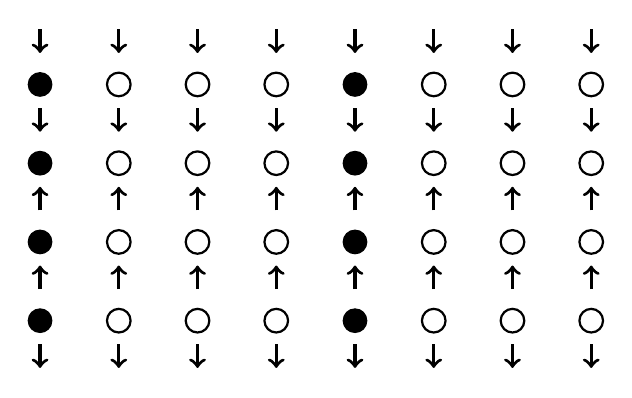
\begin{tikzpicture}
    % charge stripe
    \foreach \y in {0,1,2,3} {
        \foreach \x in {0,4} {
            \filldraw (\x+0,\y) circle [radius=0.15];
            % afm
            \draw [thick] (\x+1,\y) circle [radius=0.15];
            \draw [thick] (\x+2,\y) circle [radius=0.15];
            \draw [thick] (\x+3,\y) circle [radius=0.15];
        }
    }
    
    \foreach \x in {0,1,2,3,4,5,6,7} {
        \draw [very thick, <-] (\x,-0.6) -- (\x,-0.3);
        \draw [very thick, ->] (\x,-0.6+1) -- (\x,-0.3+1);
        \draw [very thick, ->] (\x,-0.6+2) -- (\x,-0.3+2);
        \draw [very thick, <-] (\x,-0.6+3) -- (\x,-0.3+3);
        \draw [very thick, <-] (\x,-0.6+4) -- (\x,-0.3+4);
    }
\end{tikzpicture}
    \caption[2D phonon anomaly sketch]{Possible 2D real-space scenarios of a coupling between the Cu-O bond-stretching phonon at $q=(0.25,0.25,0)$ and stripe order. Here, the phonon wavector is perpendicular to the stripe direction (parallel to the stripe propagation vector). Small arrows represent displacement of oxygen atoms. Charge oscillations are phason modes of the stripes and the black bars represent charge domain walls. The Lower figure refers to a situation where static charge order lowers the energy of the phonon (intuitively through the change of spring constant). open circles represent hole-poor anti-ferromagnetic Cu atoms and filled circles represent hole-doped ($\frac{1}{2}$ hole per site) Cu atoms.}
    \label{fig:anomaly_1d}
\end{figure}

\begin{figure}
    \centering
    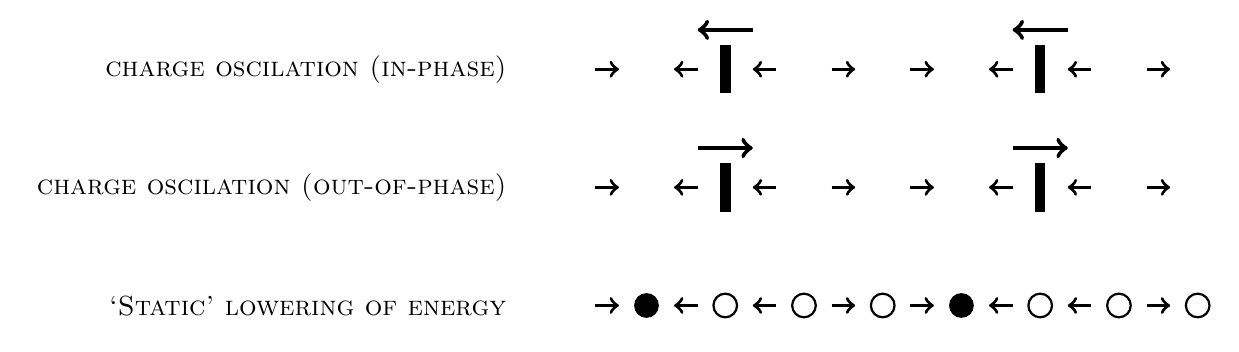
\begin{tikzpicture}
    % domain wall movement
    \foreach \y in {1.5,3} {
        \foreach \x in {0,4} {
            \draw [->, very thick] (\x,\y) -- (\x+0.3,\y);
            \draw [<-, very thick] (\x+1,\y) -- (\x+1.3,\y);
            \draw [<-, very thick] (\x+2,\y) -- (\x+2.3,\y);
            \draw [->, very thick] (\x+3,\y) -- (\x+3.3,\y);
        }
    }
    % domain walls
    \filldraw (1.59, 1.2) rectangle (1.71, 1.8);
    \draw [->, ultra thick] (1.3,2.0) -- (2.0,2.0);
    \filldraw (1.59+4, 1.2) rectangle (1.71+4, 1.8);
    \draw [->, ultra thick] (1.3+4,2.0) -- (2.0+4,2.0);
    \filldraw (1.59+4, 1.2+1.5) rectangle (1.71+4, 1.8+1.5);
    \draw [<-, ultra thick] (1.3,2.0+1.5) -- (2.0,2.0+1.5);
    \filldraw (1.59, 1.2+1.5) rectangle (1.71, 1.8+1.5);
    \draw [<-, ultra thick] (1.3+4,2.0+1.5) -- (2.0+4,2.0+1.5);
    
    % charge stripe
    \foreach \x in {0,4} {
        \draw [->, very thick] (\x,0) -- (\x+0.3,0);
        \draw [<-, very thick] (\x+1,0) -- (\x+1.3,0);
        \draw [<-, very thick] (\x+2,0) -- (\x+2.3,0);
        \draw [->, very thick] (\x+3,0) -- (\x+3.3,0);
        % charge
        \filldraw (\x+0.65,0) circle [radius=0.15];
        % afm
        \draw [thick] (\x+1.65,0) circle [radius=0.15];
        \draw [thick] (\x+2.65,0) circle [radius=0.15];
        \draw [thick] (\x+3.65,0) circle [radius=0.15];
    }
    
    \node [left] at (-1,0) {\textsc{`Static' lowering of energy}};
    \node [left] at (-1,1.5) {\textsc{charge oscilation (out-of-phase)}};
    \node [left] at (-1,3.0) {\textsc{charge oscilation (in-phase)}};
\end{tikzpicture}
    \caption[1D phonon anomaly sketch]{Possible 1D (Kohn Anomaly) scenario of the phonon anomaly. In this case the phonon wavevector resonates with the charge component parallel to the the stripes (perpendicular to the stripe propagation vector).}
    \label{fig:anomaly_2d}
\end{figure}

\begin{figure}
    \centering
    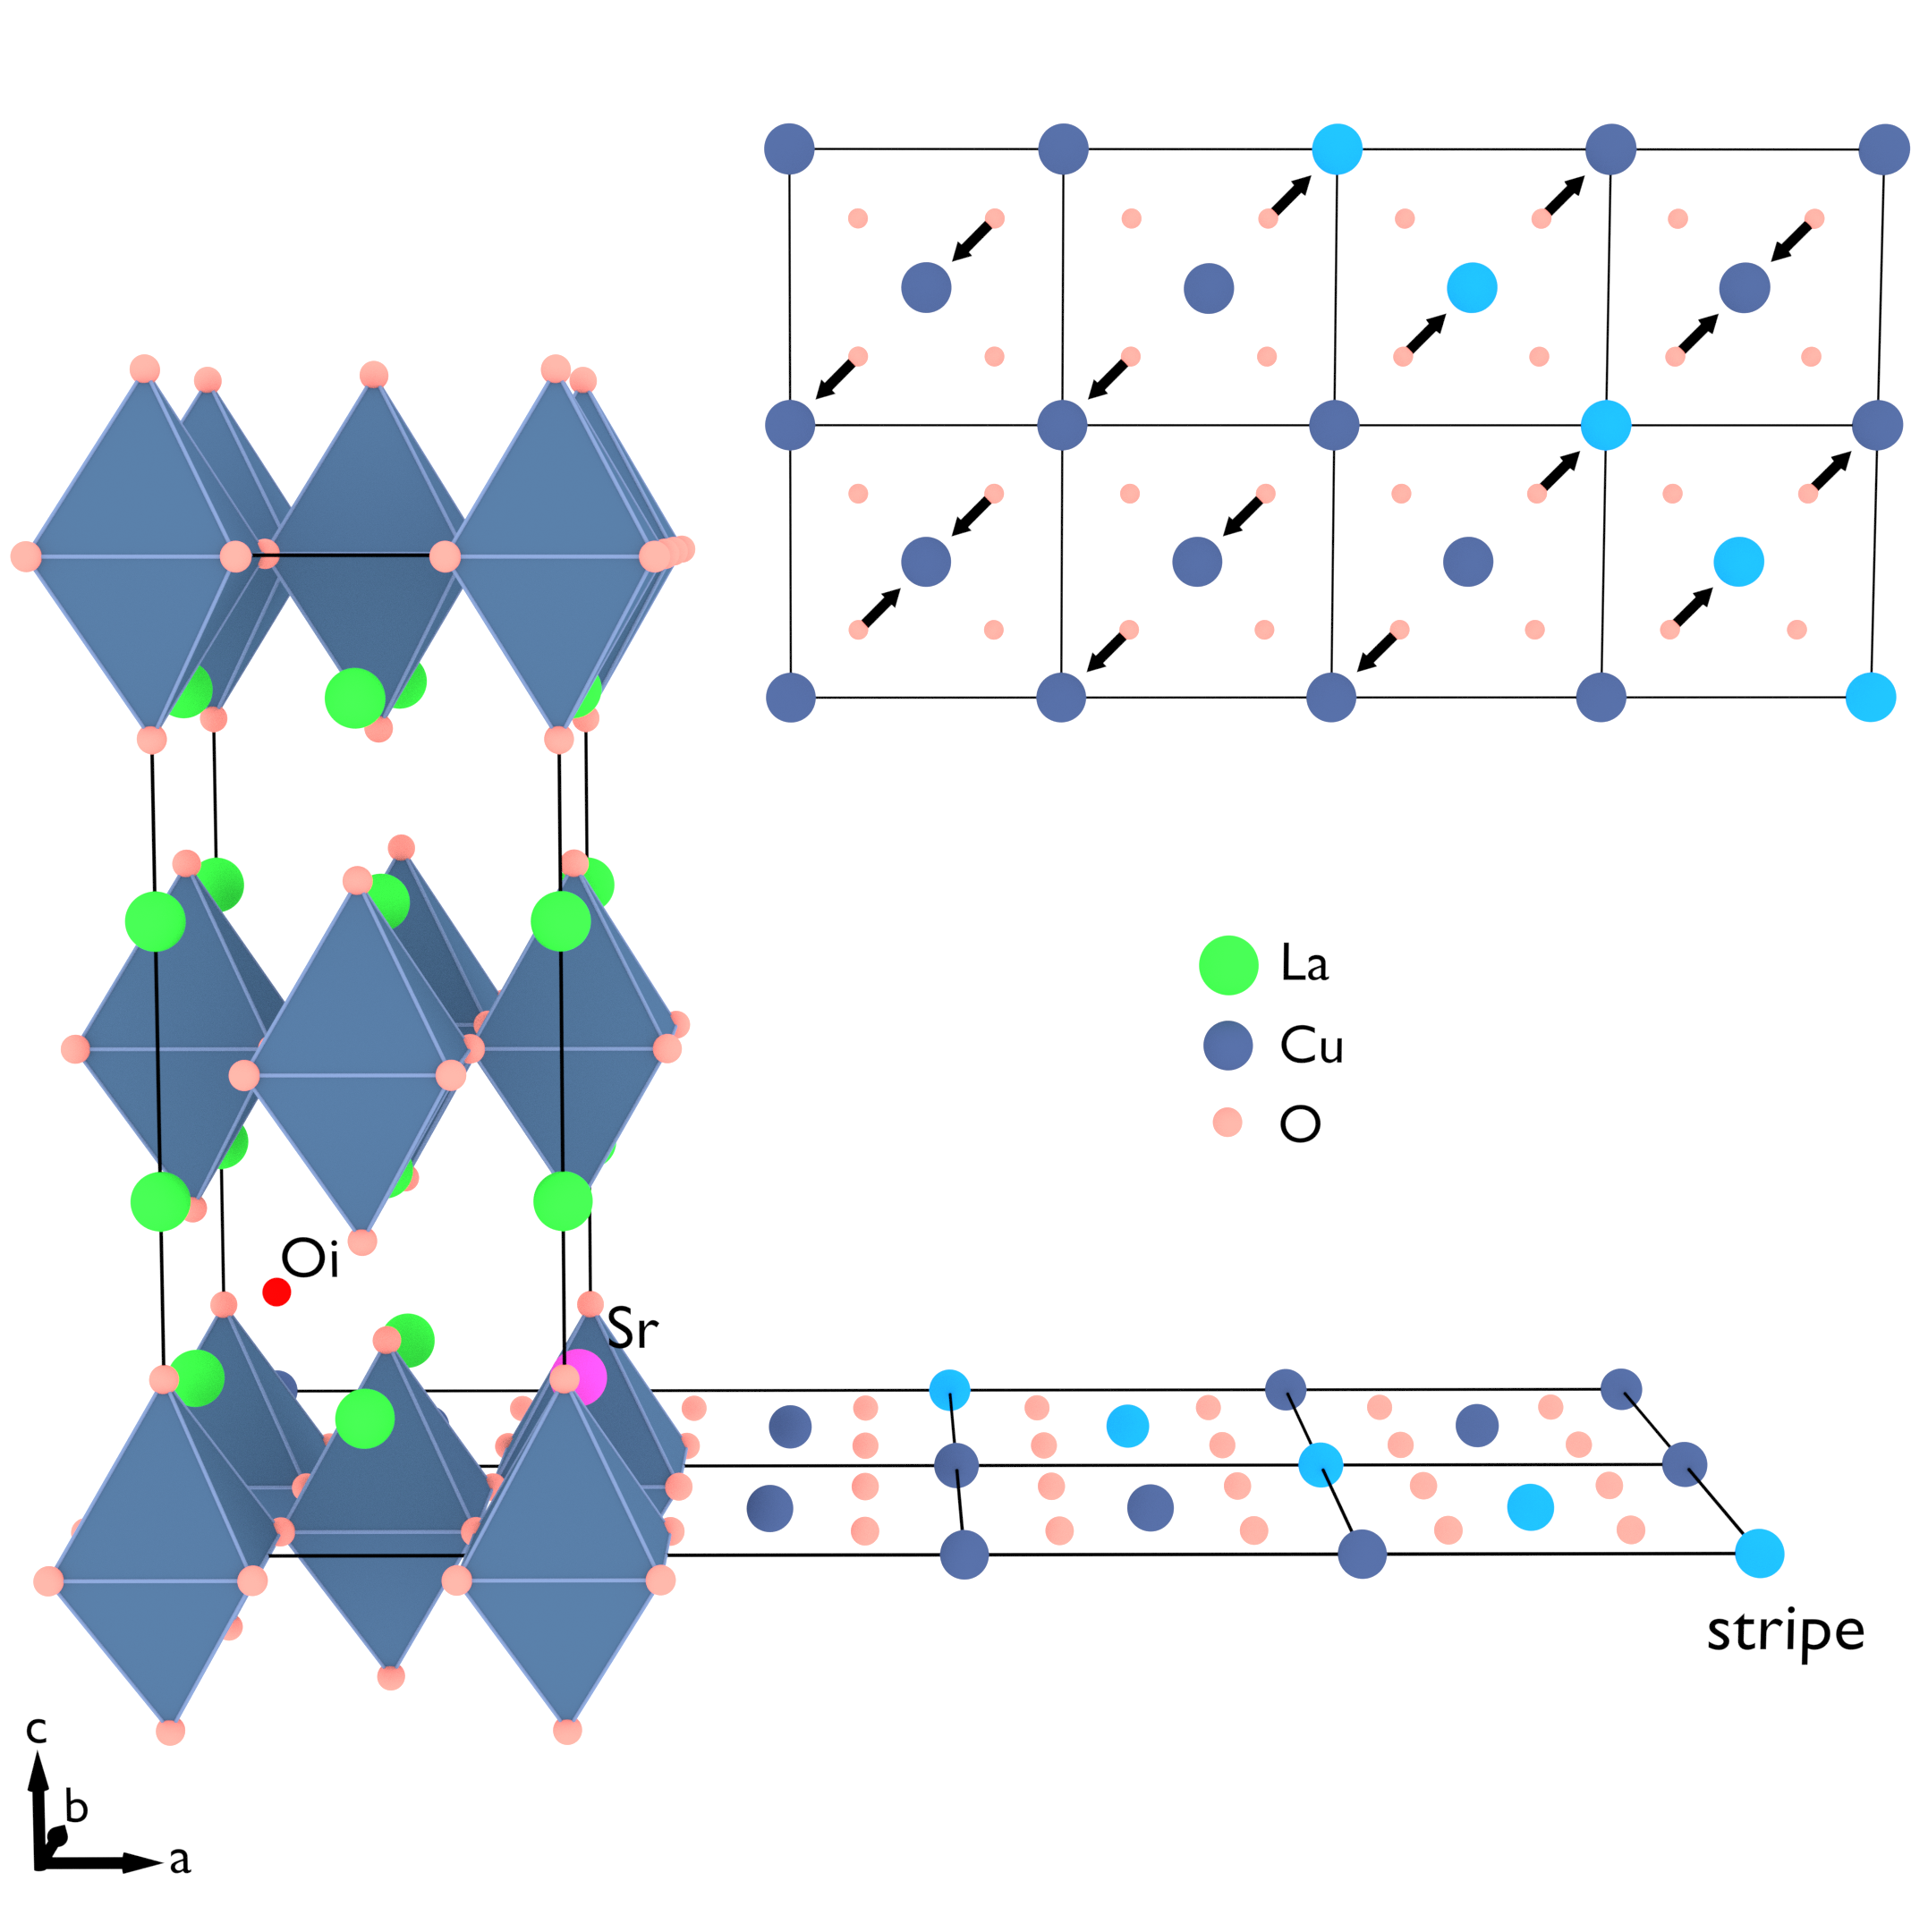
\includegraphics[width=0.7\textwidth]{fig/anomaly/overview.png}
    \caption[Crystal structure annotated with phonon at (0.25,0.25,0) and stripe order]{Sketch of crystal LSCO+O crystal structure containing two distinct dopants in a $4 \times 2 \times 1$ orthorhombic unit cell. The two singular Sr/O dopants correspond to a hole doping of $n_h = \frac{3}{32} \approx 0.09$. Dark blue are magnetic Cu sites while light blue represents hole-rich Cu sites. This period-4/8 segregation into charge/magnetic regions is known as stripe formation \cite{Tranquada1995}. Inset: Possible matching of stripe dynamics with the Cu-O bond stretching mode at q=$(0.25,0.25,0)$ as proposed by \citeauthor{Kaneshita2002} \cite{Kaneshita2002}.}
    \label{fig:crystal_anomaly}
\end{figure}

\begin{figure}
    \centering
    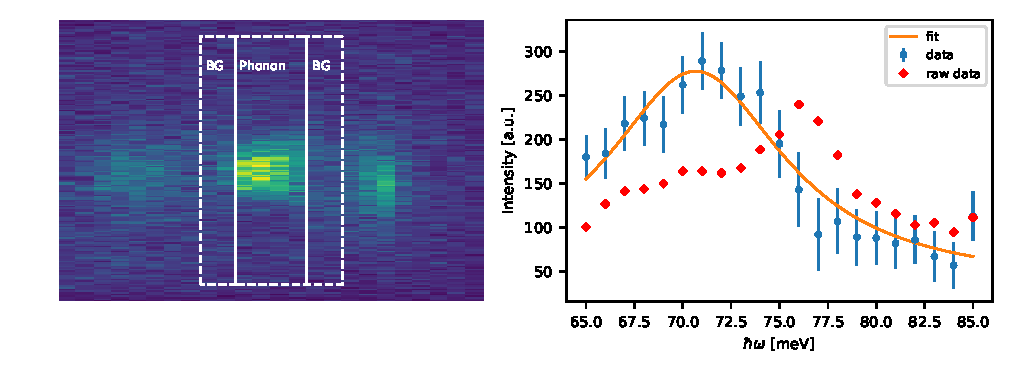
\includegraphics[width=0.54\textwidth]{fig/anomaly/data_reduction.pdf}
    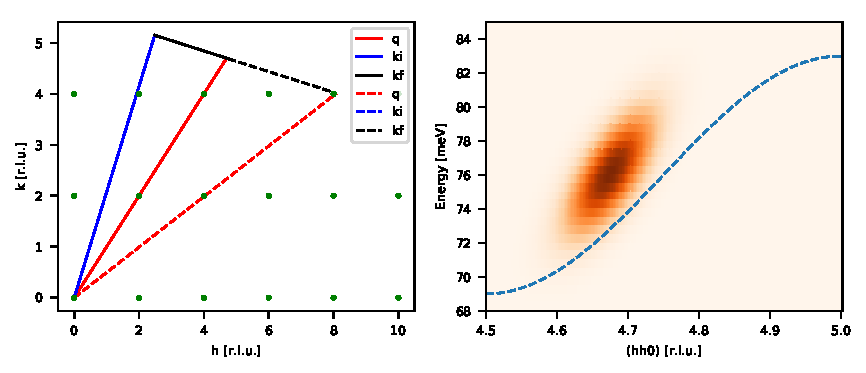
\includegraphics[width=0.45\textwidth]{fig/anomaly/spurion.pdf}
    \caption[IMPS data reduction and Spurion vizualisation]{\textbf{Top-left:} Raw data (summed from one constant-$Q$ scan) from the IMPS 2D detector. The phonon signal is observed in the central area and spurious signal is seen towards the edges. Broken white lines mark the areas used for data reduction. \textbf{Bottom-left:} Result of data reduction using the defined areas. We are clearly able to separate the phonon and spurious signal with this procedure. \textbf{Top-Right:} Scattering triangle responsible for the A-type spurious scattering (broken lines) at $Q=(4.7,4.7,0)$. The culprit is the (8,4,0) reflection. \textbf{Bottom-right:} Simulated effect of the (8,4,0) reflection on a $Q$-$\hbar\omega$ map assuming a Gaussian spurious signal depending on distances in $Q$. Broken line represents a `normal' (not anomalous) dispersion in this region.}
    \label{fig:imps_data_reduction}
\end{figure}

\begin{figure}
    \centering
    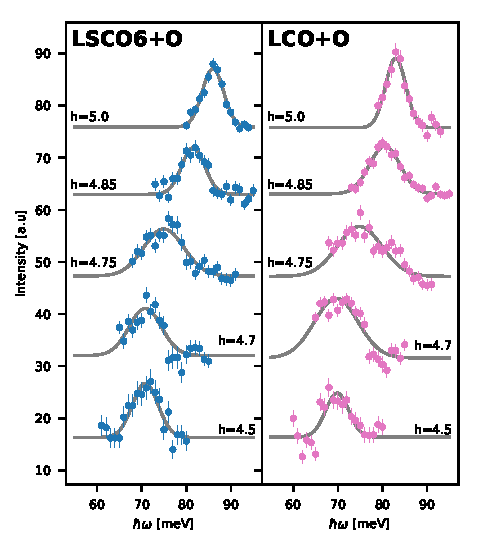
\includegraphics[width=0.49\textwidth]{fig/anomaly/selected.pdf}
    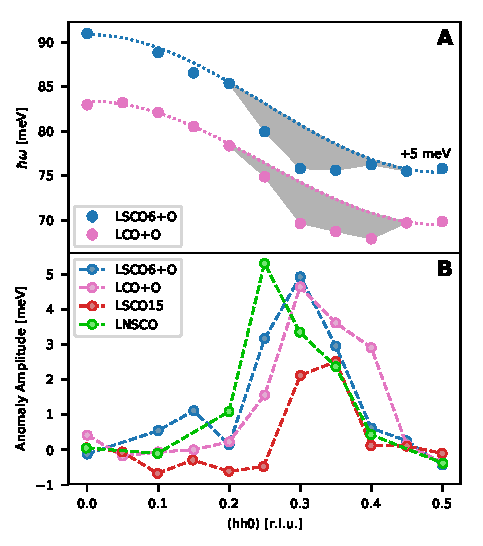
\includegraphics[width=0.49\textwidth]{fig/anomaly/disp_aa_2.pdf}
    \caption[Phonon anomaly data and dispersion]{\textbf{Left:} Raw data for LSCO6+O and LCO+O obtained with IMPS detector at IN8, ILL. Fits to Gaussian lineshape. \textbf{Right:} (A) Dispersion of LSCO6+O and LCO+O obtained from peak positions of the raw data. (B) Comparison of the anoamly amplitude (shaded gray area) between LSCO6+O, LCO+O, LSCO15 ($T_\text{c} \approx \SI{40}{\kelvin}$) and LNSCO ($x=0.12$, insulating).}
    \label{fig:anomaly_rawdata}
\end{figure}

\begin{figure}
    \centering
    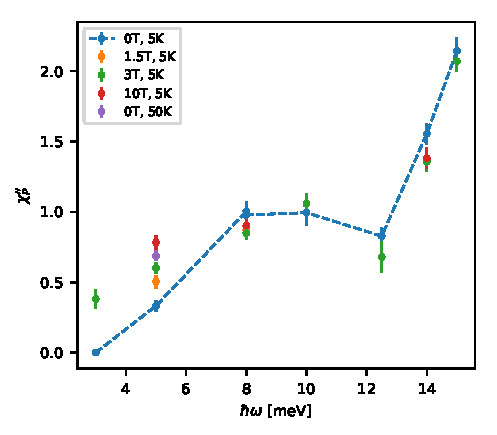
\includegraphics[width=0.49\textwidth]{fig/anomaly/chi.pdf}
    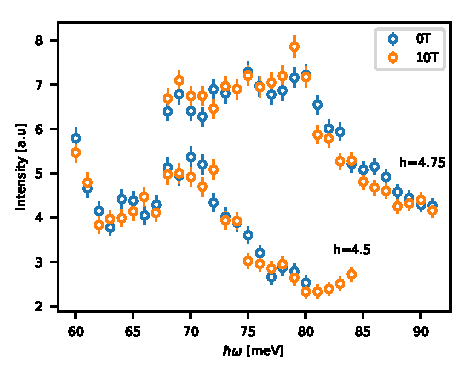
\includegraphics[width=0.49\textwidth]{fig/anomaly/field_selected.pdf}
    \caption[LSCO6+O magnetic field effect on fluctuations and phonon]{\textbf{Left:} Imaginary part of the magnetic susceptibility in LSCO6+O as a function of energy transfer, field and temperature. As shown, a field of \SI{3}{\tesla} is sufficient to open a gap in the magnetic excitation spectrum. \textbf{Right:} Raw phonon data at anomalous ($h=4.75$) and normal $h=4.5$ wave vectors as a function of field. Contrary to the magnetic excitation spectrum, the anomalous phonon does not appear to be modified by an applied field.}
    \label{fig:phonon_chi_field}
\end{figure}
